\chapter{Design}
\label{ch:design}

This chapter discusses the whole design of the system, containing the overall design and the detailed description of each part of the system. 

\section{Overall Design}
To meet the requirements of the project, the general design of the system can be divided into three parts: input data, clustering model and output result. COVID-19 related documents from Twitter would be regarded as the input dataset of the system. The system can be treated as a black box and the NLP topic model and additional analysis of the generated topics can be the representation for this black box. Additionally, the output is the analyzing result from the potential topics of the input data, which is ultimately what we want in our system. 

\begin{figure}[H]
    \centering
    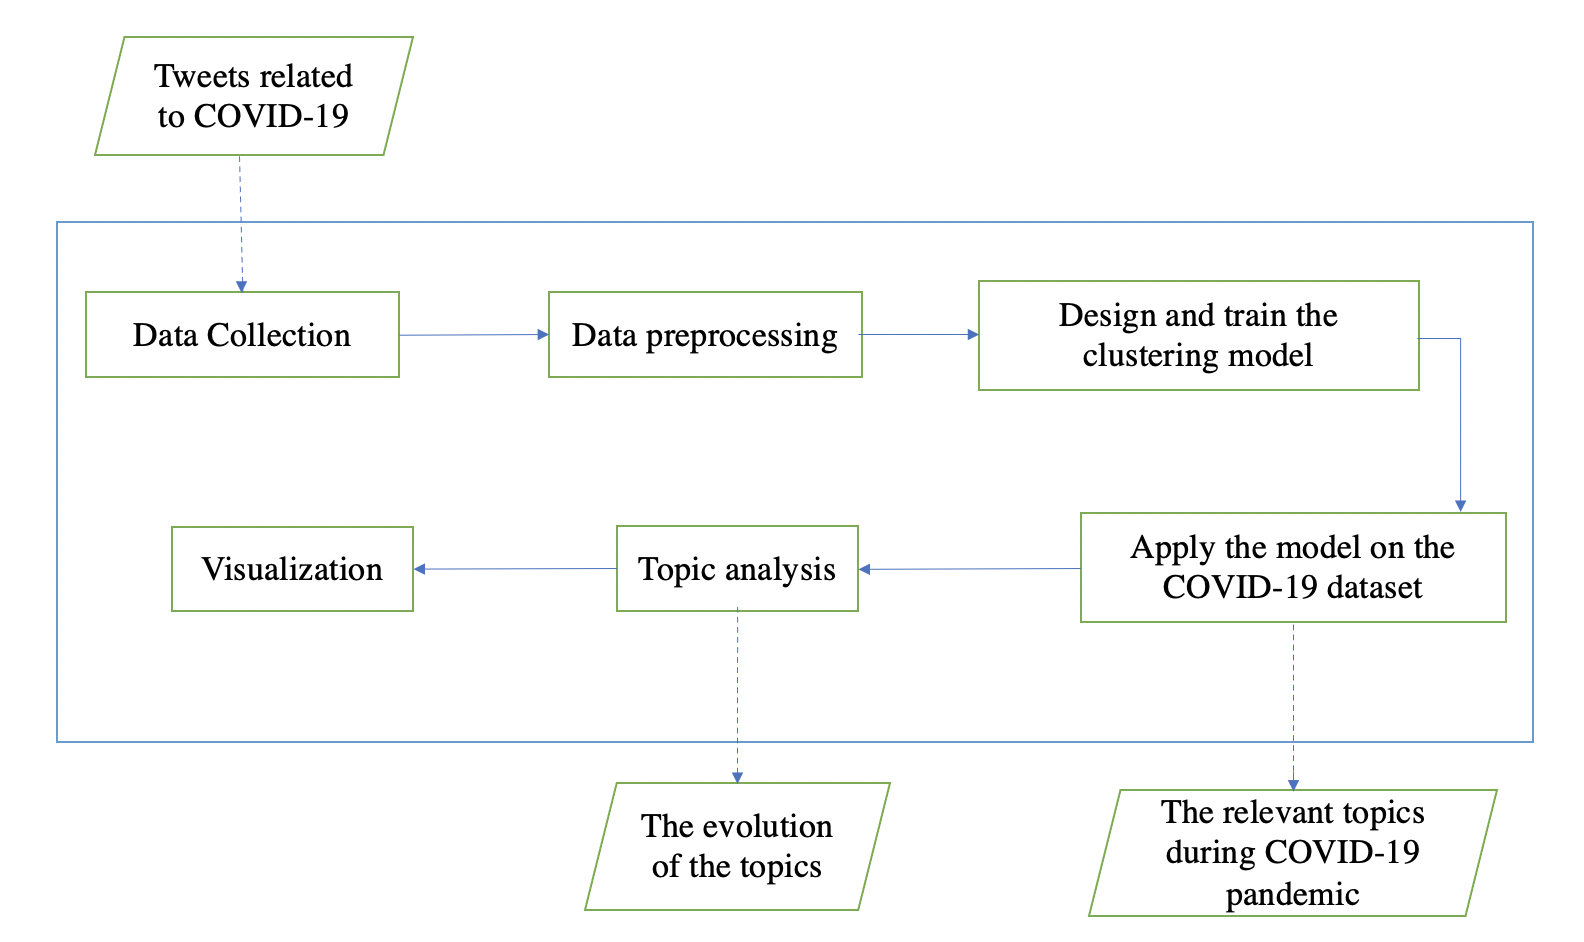
\includegraphics[scale=0.4]{images/overall_design.png}
    \caption{Overall Design}
    \label{fig:1}
\end{figure}

The above figure \ref{fig:1} shows the general graphical structure of the system design, where the rectangles represent the main steps, and the parallelograms with the dashed arrow represent the input or products of those steps. And the main process for the implementation is: 1) data collection, 2) data preprocessing, 3) select the appropriate model to cluster the texts documents, 4) applying the model to the dataset and generate the result, 5) topic analysis, and 6) show the visualization result. 

\section{Basic Components Design}
The design of the basic components in the system is discussed in this section and it will include the functional design of each part and why it suit the project.


\subsection{Data Collection} \label{collection}
Twitter data is chosen as the input social media data of the whole system. Crawling Twitter data can be implemented by an official Twitter API or directly download from an open source website. When designing the data collector, four requirements should be considered:

\begin{enumerate}
    \item The collected Tweets should be written in English since this project focus on English Tweets analysis.
    \item Besides the main body of the Tweet,   the username, Tweet created time and location should also be collected to complete the dataset.
    \item The created time of the collected Tweet should be during the COVID-19 pandemic.
    \item The contents of the collected Tweets should be related to COVID-19.
\end{enumerate}

\subsection{Data Preprocessing} \label{preprocessing}
The collected data can not be directly used in the clustering model since the structures of social media data mainly from unstructured user grammar so that structures are complex and irregular \cite{abidin2019model}. Therefore, after collecting data at stage 1, the original dataset should be preprocessed to make it suits for the clustering model.

The following shows the basic steps of preprocessing:

\begin{enumerate}
    \item Structure unification: the media social data may be from different sources with different data structures. If those data should be regarded as the input of the later model training, there is a uniform structure requiring. In addition to the necessary information mentioned before, the dataset can also contain information that would not be used at the current stage, in case need it later.
   
    \item Data regularization: the collected Twitter data might contain some noise information such as emoji, URL, pictures, and videos, but we primarily focus on the pure text. So, in this step, that noise information would be ignored, and the emoji would be replaced by the corresponding regular text. 
   
    \item Stemming: since the algorithm will be modeling on the words in the document, the unification of a word is significant. Stemming is unifying the various forms of a word into one common representation \cite{vijayarani2015preprocessing}. For example, words: 'interesting', 'interested', 'interests' should all be represented as 'interest'. 
    \item Removing: because of the particularity of text data, there are some features might influence the accuracy of the clustering model. For example, stop words such as 'are', 'and' are not useful for the analysis of the documents and should be removed. Also, social network users prefer to use slang in their texts, such as '4u' means 'for you', '2day' means 'today'. These slangs should also be filtered and translated to their basic form. Moreover, punctuations should also be deleted.
   
    \item Tokenization: the task of tokenization is to split the text data into units (tokens), which is one of the early processing steps of NLP \cite{grefenstette1999tokenization}. There are three types of separation of texts: split texts into words, into single characters and split texts into sub-word (n-gram). Since our algorithm will be modeling on words, we adopt the word-tokens strategy.
    
    \item Data filter: after the above steps, if the document remains less than three words, it could be treated as useless data, which should be filtered. 
\end{enumerate}

\subsection{Clustering Model}

Some NLP topic models can be used as the clustering model in our system to excavate the main topics of the input documents. The followings are the functional requirements of the model:

\begin{enumerate}
    \item The filtered data should be generated from the clustering model and should be assigned into clusters.
    \item Each cluster should have an explainable topic.
\end{enumerate}

\subsection{Visualization}
The visualization result mainly focuses on using interactive graphics to make user make sense about the science data on some potential features such as the relationship and the trend \cite{grinstein2002information}. For different purpose or different data type, there are various techniques for visualization including basic 2D visualization such as bar chart, 3D visualization and dynamic visualization. In this project, there are two types of visualization should be shown:

\begin{enumerate}
    \item The visualization result should show the details of the topics, for example, display the top words in each topic.
    \item The visualization result should show the topic distribution and variation during the pandemic.
\end{enumerate}

Word cloud has become a visually attractive and straightforward method of text visualization, which display the highest frequency words in a text to represent the overview of the text \cite{cui2010context}. As figure \ref{fig:2} shows, it is satisfied for topic visualization. Traditional bar chart can distinct demonstrate the distribution of the topics, and the example is as figure \ref{fig:3}.

\begin{figure}[H]
    \begin{minipage}[t]{0.4\linewidth}
        \centering
        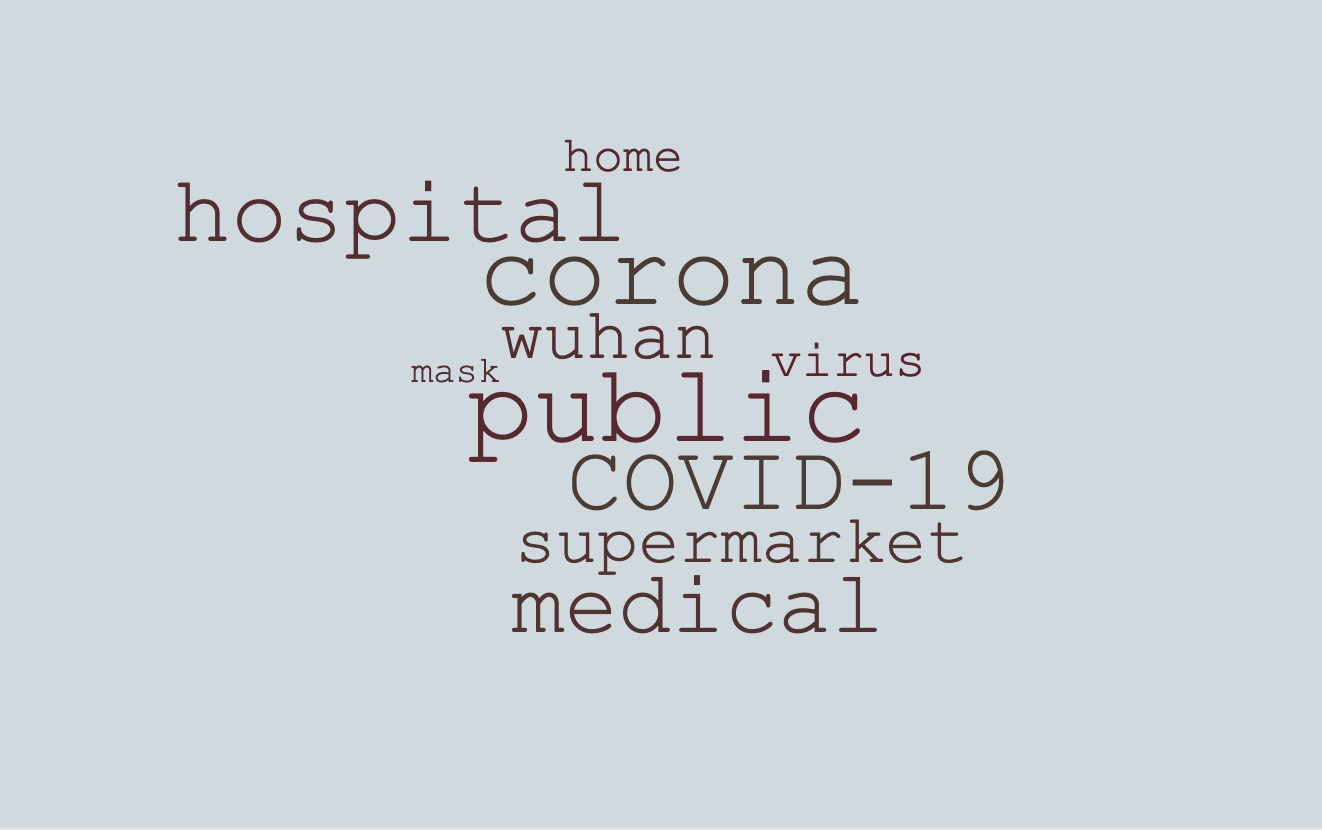
\includegraphics[scale=0.2]{images/visualization_exp1.png}
        \caption{Word Cloud}
        \label{fig:2}
    \end{minipage}%
    \begin{minipage}[t]{0.5\linewidth}
        \centering
        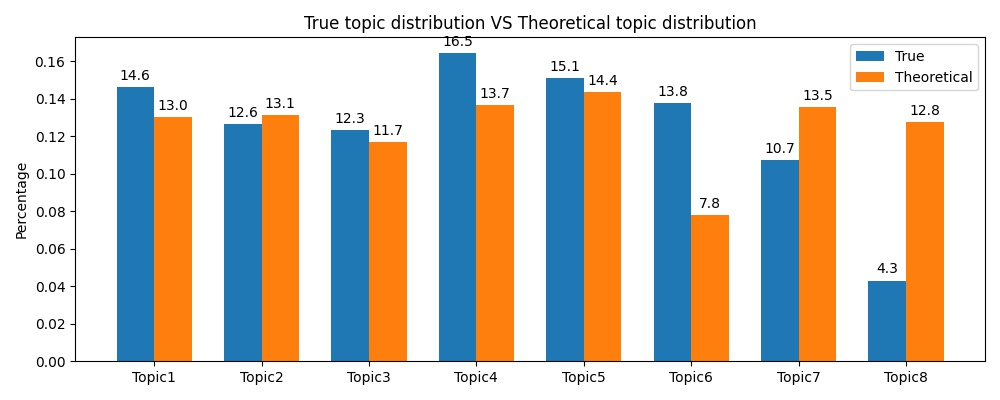
\includegraphics[scale=0.3]{images/visualization_exp2.jpg}
        \caption{Bar Chart}
        \label{fig:3}
    \end{minipage}
\end{figure}

\section{Algorithm Design Specification}\label{model_design}
In Chapter 2, there are three different algorithms, K-means, LDA and BTM, are introduced that can be used in this project for text clustering. In the early stage of the project, the exploration of suitable clustering model started from K-means, then tried LDA and BTM respectively, and finally designed our own model based on BTM. This section focuses on the specific design of our model Triterm Topic Model(TTM). Since TTM is a modified BTM, the design details of BTM are also discussed.

\subsection{BTM}
The purpose is to train the parameters $\vec\varphi_1,...,\vec\varphi_K$ and $\vec\theta_1,...,\vec\theta_M$, and using the model to compute a new topic-word distribution $\vec\theta_new$ for a new document. A plentiful enough corpus will be used as the training dataset to inference the Tweets related to COVID-19. 

The training process for BTM model is using Gibbs sampling obtained the $(z,b)$ samples in the corpus, and estimate all the parameters based on the samples. The training algorithm is as follows \cite{cheng2014btm}, where $n_k$ denotes to the number of biterms assigned to topic k, $n_{w|k}$ denotes to the number of times that word $w$ assigned to topic k, and the topic-word matrix $\vec\varphi$ is the model:

\begin{algorithm}[H]
  \SetAlgoLined
  \KwIn{topic number K, $\alpha$ and $\beta$, biterm set $B$}
  \KwOut{$\vec\theta$, $\vec\varphi$}
  Random assign a topic $z$ to all the biterms\;
  \For{$iter=1$ to $N_{iter}$}{
        \ForEach{biterm $b_i=(w_i,w_j)\in B$}{
            Draw topic $k$ from $P(z_i|z_{\lnot i},B)$\;
            Update $n_{k}$,$n_{w_i|k}$ and $n_{w_j|k}$\;
        }
    }
  compute the parameters $\vec\theta$ and $\vec\varphi$\;
  \caption{Gibbs sampling for BTM training}
\end{algorithm}

The inference process is similar to the training process. Keep the $\hat\varphi_{kt}$ in the Gibbs sampling formula unchanged from training process, then estimate the topic distribution for the new document. 

\begin{algorithm}[H]
  \SetAlgoLined
  \KwIn{topic number K, new document $d_new$, $\alpha$ and $\beta$, new biterm set $B_{new}$, $phi$}
  \KwOut{$\vec\theta_new$}
  Randomly assign a topic $z$ to all the biterms in $d_{new}$\;
  \For{$iter=1$ to $N_{iter}$}{
        \ForEach{biterm $b_i=(w_i,w_j)\in B_{new}$}{
            re-sampling the topic of $b_i$ by Gibbs sampling formula
        }
    }
  compute the topic distribution of the new document, which is $\vec\theta_{new}$\;
  \caption{Gibbs sampling for BTM inference}
\end{algorithm}

\subsection{TTM}
As illustrated in Section \ref{topicmodel}, our model Triterm Topic Model(TTM) extends modeling the biterms to triterms in the short text. 'triterm' denotes the three-word group co-occuring in the short text. For example, document$(w_1,w_2,w_3,w_4)$ will generate four triterms$\{(w_1,w_2,w_3),(w_1,w_3,w_4),(w_1,w_2,w_4),(w_2,w_3,w_4)\}$. The graphical representation of TTM is as the following figure \ref{fig:8} shows.

\begin{figure}[H]
    \centering
    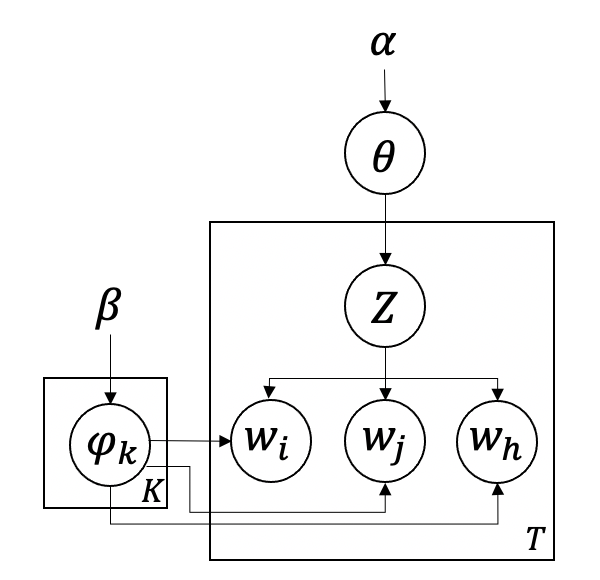
\includegraphics[scale=0.6]{images/TTM_graph.png}
    \caption{Graphical representation of TTM}
    \label{fig:8}
\end{figure}

The generative process of TTM is:
\begin{enumerate}
    \item Draw $\theta\sim Dirichlet(\alpha)$
    \item For each topic $k\in[1,K]$
    \begin{enumerate}
        \item draw $\phi_k\sim Dirichlet(\beta)$
    \end{enumerate}
    \item For each biterm $b_i\in B$
    \begin{enumerate}
        \item draw $z_i\sim Multinomial(\theta)$
        \item draw $w_i,w_j,w_h\sim Multinomial(\phi_{z_i})$
    \end{enumerate}
\end{enumerate}

The training and inference processes are very similar to BTM. For training a TTM, randomly assign a topic to each triterm. In each iteration, update the topic for each triterm by the Gibbs sampling formula and when the Gibbs sampling converges, compute the parameter $\vec\theta$ and $\vec\varphi$ then get the model. And the Gibbs sampling formula for TTM is:

\begin{equation}
     p(z_i=k|\vec z_{\lnot i},\vec t)\ \propto\ \theta_k\ \cdot\ \varphi_{k, w_i}\ \cdot\ \varphi_{k,w_j}\ \cdot\ \varphi_{k,w_h}
\end{equation}

\begin{algorithm}[H]
  \SetAlgoLined
  \KwIn{topic number K, $\alpha$ and $\beta$, triterm set $T$}
  \KwOut{$\vec\theta$, $\vec\varphi$}
  Random assign a topic $z$ to all the triterms\;
  \For{$iter=1$ to $N_{iter}$}{
        \ForEach{triterm $t_i=(w_i,w_j,w_h)\in T$}{
            Draw topic $k$ from $P(z_i|z_{\lnot i},T)$\;
            Update $n_{k}$,$n_{w_i|k}$, $n_{w_j|k}$ and $n_{w_h|k}$\;
        }
    }
  compute the parameters $\vec\theta$ and $\vec\varphi$\;
  \caption{Gibbs sampling for TTM training}
\end{algorithm}


Also the formula for parameter updating is as follows, where $n_{w|k}$ denotes the number of times that word $w$ assigned to topic $k$, $n_k$ denotes to the number of triterms in topic $k$ and $N_T$ is the number of all triterms.

\begin{equation}
\begin{aligned}
    \varphi_{k,w}\ &=\ \frac{n_{w|k}+\beta}{\sum_{w} n_{w|k}+W\beta}\\
    \theta_k\ &=\ \frac{n_k+\alpha}{N_T+K\alpha}
\end{aligned}
\end{equation}

The process of TTM inference is designed as follows:

\begin{algorithm}[H]
  \SetAlgoLined
  \KwIn{topic number K, new document $d_{new}$, new titerm set $T_{new}$, $\alpha$ and $\beta$, $\vec\phi$}
  \KwOut{$\vec\theta_{new}$}
  Random assign a topic $z$ to all the triterms in $d_new$\;
  \For{$iter=1$ to $N_{iter}$}{
        \ForEach{titerm $t_i=(w_i,w_j,w_h)\in T_{new}$}{
            re-sampling the topic of $t_i$ by Gibbs sampling formula
        }
    }
  compute the topic distribution of the new document, which is $\vec\theta_{new}$\;
  \caption{Gibbs sampling for TTM inference}
\end{algorithm}
